\chapter{Generative Pattern Database}

Three main challenges in the context of data dissemination in CIDS were identified. First, intrusion related data is usually of sensitive nature. Thus, the exchange mechanism must not compromise \textit{privacy} policies and regulations. At the same time, the usability of the data has to be preserved. Second, the data that is subject of the exchange may exhibit large volumes. That constitutes a challenge, since the dissemination is desired to be executed with a \textit{minimal overhead} in a timely and scalable fashion. Lastly, the \textit{interoperability} of the CIDS with existing local IDS is an important aspect that influences the adoption and operational usability in practice. 

In summary, existing approaches for data dissemination mainly provide mechanisms for exchanging alert data or single attributes, e.g. IP addresses, as they focus on the correlation of intrusion detection incidents that originate from different sensors. The exchange of actual training data is neglected, possibly due to high data volumes. Thus, these systems lack of mechanisms for the extraction and global persistence of novel attack patterns, e.g. zero day exploits, that can be used for the training of an intrusion detection sensor.

The approach that is presented in this chapter exchanges attack patterns by sharing generative machine learning models that have been trained on partitions of similar data points. Such a model-based dissemination enables the receiving side to sample a synthetic dataset that enhances existing local datasets. This provides two main advantages. First, no original data leaves a local network and therefore does not violate any privacy restrictions. Second, the data is compressed considerably by representing it in form of a generative model. In order to make that mechanism scalable, the monitored data is clustered using random projections. This way, similar data points are partitioned into globally common clusters and provide data parallelism, such that updates on the database is done efficiently in a cluster-wise fashion. Furthermore, this mechanism enables a similarity-based correlation of distributed intrusion events. The integration of both a similarity based correlation of intrusion incidents and a mechanism for sharing attack knowledge makes it possible to extract novel patterns of distributed attacks and provide them globally within the CIDS, resulting in an improved attack detection.

While Section \ref{sec:system_architecture} gives a high-level overview of the proposed architecture and its main processing primitives, details on the specific algorithms and strategies of the main services are described in Sections \ref{sec:local_indexing} to \ref{sec:classifier_fitting}.

\section{System Architecture} \label{sec:system_architecture}

% Provide a general view on main components and their tasks and interfaces; how is this system supposed to work; how do the components interact with each other
% Specify important definitions on components and data formally


\begin{figure}[b!]
    \centering
    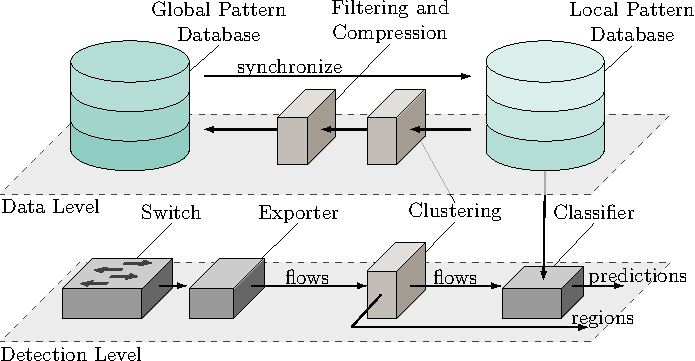
\includegraphics[width=1\linewidth]{tikz/high_level_architecture.pdf}
    \caption{High level CIDS architecture.}
    \label{fig:high_level_architecture}
    \end{figure}

    
    Logically, the proposed CIDS exhibits a hierarchical architecture (see Figure \ref{fig:high_level_architecture}). For one, the global infrastructure $G$ represents the collection of $M \in \mathbb{N}$ CIDS participants and their knowledge on an abstract level. For another, it provides specific services, that are globally available to each local infrastructure $L_m, m \in \{1, \dots, M\}$ that includes all CIDS components and processes within the IT infrastructure boundaries of a corresponding CIDS member. Each local infrastructure $L_m$ agrees to a specified feature extraction process that provides the monitoring data $\bm{X} \subset \mathbb{R}^d$ for the attack detection. Single data points of the monitoring data are referred to as $\bm{x} \in \bm{X}$ with a total number of features $d = |\bm{x}| \in \mathbb{N}$. In addition, the set of targets $Y \subset \mathbb{N}$ with instances $y \in Y$ is known and registered by every local infrastructure $L_m$. Furthermore, every $L_m$ prodives an individual training dataset $D_m= \{(\bm{x}_n, y_n): 1 \leq n \leq N_m\}$ of size $N_m = |D_m| \in \mathbb{N}$. CIDS communication across local boundaries occurs exclusively in a vertical direction. Thus, the exchange of information between individual $L_m$ takes place indirectly via the global pattern database $(PDB_G)$ and the global event channel $(C_G)$. Each $L_m$ includes a local pattern database $(PDB_{L_m})$, a local event channel $(C_{L_m})$ and an event-based data processing pipeline that consists of four services.

    \begin{table}[b]
        \centering
        
\begin{tabular}{ll} 
    \toprule
    \textbf{Notation} & \textbf{Description}             \\ 
    \midrule
    $G$                     & Global Infrastructure            \\
    $L_m$                   & Local Infrastructure $m$             \\
    \midrule
    $PDB_G, PDB_{L_m}$                   & Global Pattern Database, Local Pattern Database of $L_m$             \\
    $C_G, C_{L_m}$                     & Global Event Channel, Local Event Channel of $L_m$                    \\
    \midrule
    $M \in \mathbb{N}$      & Total number of CIDS participants         \\
    $m \in \{1, \dots, M\}  $         & Local Infrastructure Identifier  \\
    \bottomrule
\end{tabular}

        \caption{Summary of the architecture notation.}
    \end{table}

\subsection{Pattern Database} \label{subsec:pattern_database}

% what are the tasks of a pdb
depending on the scope (either local or global), different tasks are considered
local pdbs store intrusion detection datasets and corresponding metadata of the respective member; 
global pdbs store global metadata (combined information of local datasets) and the generative models


Each instance of a pattern database $(PDB)$ is realized as a key-value store. For the following algorithm descriptions, a $PDB$ is treated as a hash table as defined in Section \ref{subsec:hash_table}, that is referred to by replacing its function variable with the identifier of the corresponding database, e.g. $PDB_G(k)$ being a specific slot or hash value related to a key $k$ in the global pattern database. Note that if a specific hash function is already used to construct a key (e.g. Random Projection), the hash table will internally apply a distinct hash function on the key to ensure even distribution across the slots.

\subsection{Event Channel} \label{subsec:event_channel}
Event channels provide a topic-based publish-subscribe messaging mechanism that is mainly used to distribute workloads among the service instances in the processing pipeline. Via the messaging system, service instances receive and emit events, on which upon the respective operations are triggered. Changes in a pattern database result in responses that in turn are leveraged as the respective events. In this fashion, updates are propagated throughout the processing pipeline, ensuring a timely consistency among the pattern databases.

\subsection{Processing Pipeline} \label{subsec:processing_pipeline} 
Local and global pattern databases serve exclusively as data sources and sinks for operations. The only exception is the initial import of datasets $D_m$ into the \textit{Local Indexing} service via the messaging system.

\section{Local Indexing} \label{sec:local_indexing}

\begin{figure}[b]
    \centering
    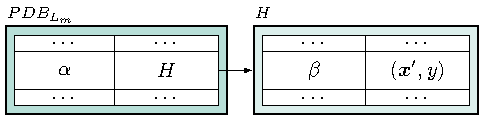
\includegraphics[width=1\linewidth]{tikz/indexing.pdf}
    \caption{Nested indexing in a local pattern database.}
    \label{fig:indexing}
\end{figure}

The local indexing service listens on $C_{L_m}$ for new data points from $D_m$. First, data points are buffered until a defined batch size is released. Subsequently, the batch $X$ is scaled to the range $[-1, 1]$ by applying a feature-wise min-max normalization, given by

\begin{align*}
    \bm{X}' = \frac{\bm{X}-min(\bm{X})}{max(\bm{X}) - min(\bm{X})} \cdot (b - a) + a, \quad
    \setlength\arraycolsep{2pt}
    \begin{array}{lr}
        a = &-1 \\
        b = & 1    
    \end{array}.
\end{align*}

After that, each element $\bm{x}' \in \bm{X}'$ is subject to both a \textit{GRP} $h$ with a global seed for the initialization of the projection plane $\bm{M}$ (see Section \ref{subsec:gaussian_random_projection}) and a non-cryptographic hashing function $g$ (see Section \ref{subsubsec:non-cryptographic-hashes}). The \textit{GRP} clusters the data by mapping similar data points $\bm{x}'$ to the same hash value. The non-cryptographic hashing function on the other hand serves as a mechanism for deduplicating identical $\bm{x}'$. In order to insert a pair $(\bm{x}'_n, y_n) \in D_m$ into the $PDB_{L_m}$, at first two keys $k_\alpha, k_\beta \in K$ are constructed as

\begin{align*}
    k_\alpha(\bm{x}'_n, y_n) &= p_x \doubleplus h(\bm{x}'_n) \doubleplus y_n,\\
    k_\beta(\bm{x}'_n) &= g(\bm{x}'_n),
\end{align*}

where $\doubleplus$ indicates the concatenation operator and $p_x$ describes an arbitrary prefix constant. Secondly, if not already present, a hash table $T_{m_n}$ is created and inserted into the slot $PDB_{L_m}(k_\alpha(\bm{x}'_n, y_n))$. Finally, $(\bm{x}'_n, y_n)$ is hashed into the slot $T_{m_n}(k_\beta(\bm{x}'_n))$. That nested indexing is depicted in Figure \ref{fig:indexing}. Since a particular $h(\bm{x}')$ is a cluster of similar data points, we refer to it as a \textit{region}. Therefore, every region is represented by one or more hash tables $T_{m_n}$, each of them containing data points that belong to the same label. Each execution of that insert operation is executed idempotently, such that the pattern database only returns a response upon the insertion of new data points. For each response, the corresponding region $h(\bm{x}'_n)$ is sent into the local event channel $C_{L_m}$ as an event that indicates a change on a certain cluster within the local pattern database.

\section{Complexity Estimation} \label{sec:complexity_estimation}

A region is said to be complex, if it contains more than one unique label. Otherwise, a region is simple. Since the data within a region already represents a cluster, the existence of multiple classes indicates a more complex decision boundary. On that basis we differentiate how a region is processed in the subsequent services of the pipeline. Furthermore, the complexity state of a region may vary, depending on the scope it is observed. Note that since the projection matrix $\bm{M}$ is initialized with the same values in every $L_m$, all hashes that were computed by $h$ are globally comparable. This means that similar data points from different datasets, e.g. $\bm{x}_i \in D_1$ and $\bm{x}_j^* \in D_2$ may be hashed to the same region $h(\bm{x}_i) = h(\bm{x}^*_j)$. However, it is also possible that that the corresponding labels $y_i \in D_1$ and $y^*_j \in D_2$ are not equal and therefore lead to a different global view on that region's complexity state. Given that, the complexity estimation module acts as a bridge between the local and global components and answers the question, which regions are considered to be complex in a global context. First, an event containing a region $h(\bm{x}'_n)$ is received. This event is then used for retrieving the set of unique labels $Y_{h(\bm{x}'_n)}$ for that particular region stored at $PDB_{L_m}$, which is defined as

 \begin{align*}
    \bigcup_{y \in Y} \! \Bigl\{ y_n \! \in \! \bigl\{T_{m_n}\bigl(k_\beta(\bm{x}'_n)\bigl)\bigl\} : \! T_{m_n} \! \! \in \! \bigl\{PDB_{L_m}\bigl(k_\alpha(\bm{x}'_n, y) \bigl)\bigl\}\Bigl\}.
 \end{align*}

 Next, a key $k_\gamma \in K$ is constructed by concatenating an arbitrary prefix constant $p_y$ with the region $h(\bm{x}'_n)$ and the id of the current local infrastructure $m$:

\begin{align*}
    k_\gamma(h(\bm{x}'_n), m) = p_y \doubleplus h(\bm{x}'_n) \doubleplus m.
\end{align*}

 Then, $Y_{h(\bm{x}'_n)}$ is inserted into the global pattern database at the slot $PDB_G(k_\gamma(h(\bm{x}'_n), m))$. The global complexity $c_{h(\bm{x}'_n)} \in \{0, 1\}$ is determined by combining the respective label sets from all local infrastructures and evaluating its cardinality:
 
 \begin{align*}
    c_{h(\bm{x}'_n)} = \Bigl| \bigcup_{m \in M} \Bigl\{ PDB_G\bigl(k_\gamma(h(\bm{x}'_n), m)\bigl) \Bigl\}\Bigl| > 1.
 \end{align*}

 Finally, the state $c_{h(\bm{x}'_n)}$ is inserted in the global pattern database by constructing a key $k_\kappa \in K$ with a prefix constant $p_c$ and the region $h(\bm{x}'_n)$ as

 \begin{align*}
     k_\kappa(h(\bm{x}'_n)) = p_c \doubleplus h(\bm{x}'_n)
 \end{align*}

and storing it in the slot $PDB_G(k_\kappa(h(\bm{x}'_n)))$. If the state has changed, a response is returned and the corresponding region $h(\bm{x}'_n)$ is sent as an event into the global event channel $C_G$.


\section{Generative Fitting} \label{sec:generative_fitting}



\section{Classifier Fitting} \label{sec:classifier_fitting}

